% !TeX program = xelatex 
\documentclass{hitreport}
\usepackage{url}
\usepackage{algorithm,float}  
\usepackage{algpseudocode}  
\usepackage{amsmath}
\usepackage{cite}
\usepackage{threeparttable}
\usepackage{subfig}
\usepackage{listings} %插入代码
\usepackage{xcolor} %代码高亮
\usepackage{tikz}
\usepackage{hyperref}



\lstset{numbers=left, %设置行号位置
	numberstyle=\tiny, %设置行号大小
	keywordstyle=\color{blue}, %设置关键字颜色
	commentstyle=\color[cmyk]{1,0,1,0}, %设置注释颜色
	frame=single, %设置边框格式
	escapeinside=``, %逃逸字符(1左面的键),用于显示中文
	breaklines, %自动折行
	extendedchars=false, %解决代码跨页时,章节标题,页眉等汉字不显示的问题
	xleftmargin=2em,xrightmargin=2em, aboveskip=1em, %设置边距
	tabsize=4, %设置tab空格数
	showspaces=false %不显示空格
}

\renewcommand{\algorithmicrequire}{\textbf{Input:}}  % Use Input in the format of Algorithm  
\renewcommand{\algorithmicensure}{\textbf{Output:}} % Use Output in the format of Algorithm  

\makeatletter
\newenvironment{breakablealgorithm}
  {% \begin{breakablealgorithm}
   \begin{center}
     \refstepcounter{algorithm}% New algorithm
     \hrule height.8pt depth0pt \kern2pt% \@fs@pre for \@fs@ruled
     \renewcommand{\caption}[2][\relax]{% Make a new \caption
       {\raggedright\textbf{\ALG@name~\thealgorithm} ##2\par}%
       \ifx\relax##1\relax % #1 is \relax
         \addcontentsline{loa}{algorithm}{\protect\numberline{\thealgorithm}##2}%
       \else % #1 is not \relax
         \addcontentsline{loa}{algorithm}{\protect\numberline{\thealgorithm}##1}%
       \fi
       \kern2pt\hrule\kern2pt
     }
  }{% \end{breakablealgorithm}
     \kern2pt\hrule\relax% \@fs@post for \@fs@ruled
   \end{center}
  }
\makeatother

% =============================================
% Part 0 Edit the info
% =============================================

\major{计算机科学与技术}
\name{孙骁}
\title{机器学习实验报告}
\stuid{1180300811} % 学号
\college{计算学部}
\date{2020年10月6日}
\lab{} %实验地点
\course{机器学习}
\instructor{刘扬}
% \grades{}
\expname{逻辑回归} %实验名称
% \exptype{} % 实验类型
% \partner{} % 同组学生名字
\term{2020秋季学期}

\begin{document}

\maketitle

\tableofcontents
\newpage
% =============================================
% Part 1 Header
% =============================================



% =============================================
% Part 2 Main document
% =============================================

\section{实验目的和要求}

\subsection{实验目的}
理解逻辑回归模型,掌握逻辑回归模型的参数估计算法.
\subsection{实验要求}
实现两种损失函数的参数估计
\begin{enumerate}
\item 无惩罚项,
\item 加入对参数的惩罚,
\end{enumerate}
可以采用梯度下降、共轭梯度或者牛顿法等

\subsection{实验验证}

\begin{enumerate}
\item 可以手工生成两个分别类别数据(可以用高斯分布),验证你的算法.考察类条件分布不满足朴素贝叶斯假设,会得到什么样的结果.
\item 逻辑回归有广泛的用处,例如广告预测.可以到UCI网站上,找一实际数据加以测试.
\end{enumerate}

\section{实验环境}

\begin{enumerate}
\item Anaconda 4.8.4
\item Python 3.7.4
\item PyCharm 2019.1 (Professional Edition)
\item Windows 10 2004
\end{enumerate}

\section{实验原理}

\subsection{线性分类问题}

考虑二分类问题,对于给定d个属性描述的示例$\boldsymbol{x} = \left(x_1;x_2;\cdots;x_d\right)$,其中$x_i$是$\boldsymbol{x}$在第$i$个属性上的取值.有$\boldsymbol{x} \in X$,$\boldsymbol{y}\in Y=\left\{0,1\right\}$,即构建映射$f: \ X\rightarrow Y$,即学习一个通过属性得线性组合进行预测的函数,
\begin{align}
f\left(\boldsymbol{x}\right) = w_1x_1+w_2x_2+\cdots+w_dx_d + b
\end{align}
改写成向量形式为
\begin{align}
f\left(\boldsymbol{x}\right) = \boldsymbol{w}^T\boldsymbol{x}+b
\end{align}
对于离散的二分类问题,我们需要针对示例$\boldsymbol{x}$进行类别的预测,比较两种类别的概率大小,将概率大的类别作为该示例的预测,即计算
\begin{align}
P(Y|X) = \dfrac{P\left(XY\right)}{P\left(X\right)}
\end{align}
使用贝叶斯公式展开,得到
\begin{align}
P(Y|X) = \dfrac{P\left(X|Y\right)P\left(Y\right)}{P\left(X\right)}
\end{align}
因此可以对给定的示例进行类别预测.


\subsection{朴素贝叶斯}

由于我们的目标是计算 $P\left(Y|X\right)$,又由贝叶斯定理可知,
\begin{align}
P\left(Y|X\right)=\cfrac{P\left(X,Y\right)}{P\left(X\right)}=\cfrac{P\left(X|Y\right)\cdot P\left(Y\right)}{\sum_{k}{P\left(X=x_i|Y\right)P\left(Y\right)}}
\end{align}
由于分母的 $P\left(X\right)$ 是常数,所以只需要计算分子即可,即
\begin{align}
P\left(Y=c_k\right),\  k=0,1
\end{align}
\begin{align}
P\left(X=x|Y=y_k\right)=P\left(X=x^{\left(1\right)},\cdots,X^{\left(d\right)}=x^{\left(d\right)}|Y=y_k\right), \ k=0,1
\end{align}
但是由于条件概率分布 $P\left(X=x|Y=c_k\right)$ 具有指数级数量的参数,其估计实际上是不可行的.因此,朴素贝叶斯对条件概率分布做了条件独立性的假设,由于这是一个较强的假设,由是也叫作“朴素”.

\begin{align}
	P\left( X=x\left| Y=c_k \right. \right) &=P\left( X^{\left( 1 \right)}=x^{\left( 1 \right)},\cdots ,X^{\left( d \right)}=x^{\left( d \right)}\left| Y=y_k \right. \right)\\
	&= \prod_{j=1}^n{P\left( X^{\left( j \right)}=x^{\left( j \right)}\left| Y=y_k \right. \right)}
\end{align}


朴素贝叶斯法学习的是生成数据的机制,因此是一种学习模型.条件独立假设即用于分类的特征在类确定的条件下都是条件独立的,这个假设使得整个算法变得简单,但是有时也会牺牲一些准确率.

因此,二分类的朴素贝叶斯的基本公式为
\begin{align}
P\left( Y=c_k\left| X=x \right. \right) =\frac{P\left( Y=y_k \right) \prod_j{P\left( X^{\left( j \right)}=x^{\left( j \right)}\left| Y=y_k \right. \right)}}{\sum_k{P\left( Y=y_k \right) \prod_j{P\left( X^{\left( j \right)}=x^{\left( j \right)}\left| Y=y_k \right. \right)}}},\ k=0,1
\end{align}

朴素贝叶斯分类器可以表示为
$$
y=f\left(x\right)=\arg \underset{c_k}{\max}\frac{P\left( Y=y_k \right) \prod_j{P\left( X^{\left( j \right)}=x^{\left( j \right)}\left| Y=y_k \right. \right)}}{\sum_k{P\left( Y=y_k \right) \prod_j{P\left( X^{\left( j \right)}=x^{\left( j \right)}\left| Y=y_k \right. \right)}}}
$$
注意到分母对所有的 $c_k$ 都是相同的,所以
$$
y=f\left(x\right)=\arg \underset{c_k}{\max}P\left( Y=c_k \right) \prod_j{P\left( X^{\left( j \right)}=x^{\left( j \right)}\left | Y=y_k \right. \right )}
$$

\subsection{Logistic回归问题}

Logistic回归的基本思想就是利用朴素贝叶斯的假设计算$P\left(Y|X\right)$:即利用$P\left(Y\right)$,$P\left(X|Y\right)$以及各个维度之间计算条件独立的假设来计算$P\left(Y|X\right)$.
对于二分类问题,我们求解$P\left(Y|X\right)$可以采用如下方式推导,
\begin{align}\label{equ:classify}
P\left(Y=0|X\right) = \dfrac{P\left(Y=0\right)P\left(X|Y=0\right)}{P\left(X\right)}
\end{align}
对式(\ref{equ:classify})的分母应用全概率公式展开,得到
\begin{align}\label{equ:mainequ}
P\left(Y=0|X\right) = \dfrac{P\left(Y=0\right)P\left(X|Y=0\right)}{P\left(X|Y=0\right)P\left(Y=0\right)+P\left(X|Y=1\right)P\left(Y=1\right)}
\end{align}
对式(\ref{equ:mainequ})右侧的分子分母同除$P\left(Y=0\right)P\left(X|Y=0\right)$,得到
\begin{align}
P\left(Y=0|X\right) &= \dfrac{1}{1+\dfrac{P\left(X|Y=1\right)P\left(Y=1\right)}{P\left(X|Y=0\right)P\left(Y=0\right)}}\\
&=\dfrac{1}{1+\exp\left\{\ln \dfrac{P\left(X|Y=1\right)P\left(Y=1\right)}{P\left(X|Y=0\right)P\left(Y=0\right)}\right\}}
\end{align}
由于我们做的是二分类问题,故$Y$的分布满足伯努利分布,记$\pi = \hat{P}\left( Y=1 \right) $,所以得到
\begin{align}
P\left(Y=0|X\right) = \dfrac{1}{1+\exp\left\{\ln\left(\dfrac{\pi}{1-\pi}\right) +\ln \left(\dfrac{P\left(X|Y=1\right)}{P\left(X|Y=0\right)}\right)\right\}}
\end{align}
此处我们利用朴素贝叶斯的假设,假设各个特征之间的分布条件独立,因此有
\begin{align}
P\left(Y=0|X\right) = \dfrac{1}{1+\exp\left\{\ln\left(\dfrac{\pi}{1-\pi}\right) +\sum_{i}\left(\ln \left(\dfrac{P\left(X_i|Y=1\right)}{P\left(X_i|Y=0\right)}\right)\right)\right\}}
\end{align}
此外,我们也假设各个维度的条件概率满足高斯分布,有各个维度的高斯分布函数$P\left(X_i|Y=y_k\right) = \frac{1}{\sqrt{2\pi}\sigma_i} \exp \left(\frac{-\left(x-\mu_{ik}\right)^2}{2\sigma_i^2}\right)$,将其带入,于是得到
\begin{align}
P\left(Y=0|X\right) = \dfrac{1}{1+\exp\left\{\ln\left(\dfrac{\pi}{1-\pi}\right) +\sum_{i}\left(\dfrac{\mu_{i1}-\mu_{i0}}{\sigma_i^2}X_i+\dfrac{\mu_{i0}^2-\mu_{i1}^2}{2\sigma_i^2}\right)\right\}}
\end{align}
将其转化为向量形式,可以得到
\begin{align}
P\left(Y|X=0\right) = \dfrac{1}{1+\exp\left(\boldsymbol{w}^T\boldsymbol{X}\right)}
\end{align}
其中,$\boldsymbol{w}_0 = \sum\limits_{i}^{n}\left(\dfrac{\mu_{i0}^2-\mu_{i1}^2}{2\sigma_i^2}\right)$,$\boldsymbol{w}_i = \dfrac{\mu_{i1}-\mu_{i0}}{\sigma_i^2}$,$i>0$,$\boldsymbol{X} = \left(1,X_1,X_2,\cdots,x_n\right)$,
由概率归一化的性质,我们可以得到
\begin{align}
P\left(Y=1|X\right) = \dfrac{\exp\left(\boldsymbol{w}^T\boldsymbol{X}\right)}{1+\exp\left(\boldsymbol{w}^T\boldsymbol{X}\right)}
\end{align}

对于给定的数据集,我们使用极大似然法对参数$\boldsymbol{w}$进行估计,于是有
\begin{align}
\boldsymbol{w} = \arg \underset{w}{\max}P\left(Y^n|X^n,\boldsymbol{w} \right)
\end{align}
对式子做对数变换,因此我们的目标是最小化式(\ref{equ:lw})
\begin{align}\label{equ:lw}
\mathcal{L}\left(\boldsymbol{w}\right) = \sum_{n}\left(-Y^n\boldsymbol{w}^TX+\ln\left(1+\exp\left(\boldsymbol{w}^T\boldsymbol{X}\right)\right)\right)
\end{align}
为了防止模型过拟合,我们加入超参数$\lambda$,得到式(\ref{equ:lwlam})
\begin{align}\label{equ:lwlam}
\mathcal{L}\left(\boldsymbol{w}\right) =\dfrac{\lambda}{2}\boldsymbol{w}^T\boldsymbol{w}+\sum_{n}\left(-Y^n\boldsymbol{w}^TX+\ln\left(1+\exp\left(\boldsymbol{w}^T\boldsymbol{X}\right)\right)\right)
\end{align}


\section{算法实现}
\subsection{梯度下降法}\label{sec:grad}
梯度下降法是通过迭代求目标函数最小值的一种方法,从数学上的角度来看,梯度的方向是函数增长速度最快的方向,那么梯度的反方向就是函数减少最快的方向.由于上述的两种误差函数为二次型,因此应用梯度下降求得的局部最优解即为全局最优解.

对式(\ref{equ:lwlam})中的$\boldsymbol{w}$应用梯度下降,在满足迭代误差保持在一定范围后,求得的$\boldsymbol{w}$即为多项式的系数向量. 算法伪代码如\ref{alg:gradient_descent}所示. 

由于实验一中使用的梯度下降算法较为依赖数据分布,因此实验二将梯度下降算法进行了封装,同时为了避免数据量过大导致的溢出,我们将式(\ref{equ:lwlam})进行了归一化处理,得到
\begin{align}
\mathcal{L}\left(\boldsymbol{w}\right) =\dfrac{\lambda}{2n}\boldsymbol{w}^T\boldsymbol{w}+\sum_{n}\left(-Y^n\boldsymbol{w}^TX+\ln\left(1+\exp\left(\boldsymbol{w}^T\boldsymbol{X}\right)\right)\right)
\end{align}



\begin{breakablealgorithm}
  \caption{Gradient Descent}  
  \label{alg:gradient_descent}  
  \begin{algorithmic}[1] 
    \Require  
    X,\,Y,\,penalty\_coefficient,\,learning\_rate,\,deviation
    \Ensure  
   	w\_result
   	\State Initialize X,\,Y,\,penalty\_coefficient,\,learning\_rate,\,deviation,\,data\_number,\,feature,\,feature\_number
   	\State Calculate pre\_loss
   	
   	\While{True}
   		\State Update w with new gradient
   		\State Calculate new loss
   		\If{newloss\,<\,deviation}
   			\State \textbf{break}
   		\Else
   			\If{new loss\,>\,old loss}
   				\State Make the learning\_rate half
   			\EndIf
   			\State Update loss and w
   		\EndIf
   	\EndWhile\\
   	\Return w
  \end{algorithmic}  
\end{breakablealgorithm}



\subsection{牛顿迭代法}\label{sec:newton}

牛顿迭代法的$\boldsymbol{w}$更新方式与梯度下降法较为类似,详细的更新方式如式(\ref{equ:neww})与式(\ref{equ:newww})所示.
\begin{align}\label{equ:neww}
\boldsymbol{w}^{t+1} = \boldsymbol{w}^{t} - \left(\dfrac{\partial^2\mathcal{L}}{\partial \boldsymbol{w}\partial\boldsymbol{w}^T}\right)^{-1}\dfrac{\partial \mathcal{L}}{\partial \boldsymbol{w}}
\end{align}
\begin{align}\label{equ:newww}
\dfrac{\partial^2\mathcal{L}}{\partial \boldsymbol{w}\partial\boldsymbol{w}^T} = \sum\limits_{i=1}^{n}\left(X_iX_i^T\dfrac{\exp\left(\boldsymbol{w}^TX\right)}{1+\exp\left(\boldsymbol{w}^TX\right)}\dfrac{1}{1+\exp\left(\boldsymbol{w}^TX\right)}\right)
\end{align}
算法伪代码如\ref{alg:newton}所示.



\begin{breakablealgorithm}
  \caption{Newton Iteration Descent}  
  \label{alg:newton}  
  \begin{algorithmic}[1] 
    \Require  
    X,\,Y,\,penalty\_coefficient,\,learning\_rate,\,deviation
    \Ensure  
   	w\_result
   	\State Initialize X,\,Y,\,penalty\_coefficient,\,learning\_rate,\,deviation,\,data\_number,\,feature,\,feature\_number
   	\State make pre\_loss
   	
   	\While{True}
   		\State Calculate new gradient
   		\If{the norm of new gradient\,<\,deviation}
   			\State \textbf{break}
   		\EndIf
		\State Calculate post\_w
		\State Update pre\_w and post\_w
   	\EndWhile\\
   	\Return w
  \end{algorithmic}  
\end{breakablealgorithm}





\section{实验步骤}

\subsection{生成满足特征条件独立的数据并测试}

设正例与反例的数据比为1:1,生成数据,训练集与测试集的比例为7:3,一共生成100个数据,均为二维数据,设置梯度下降算法的惩罚项为30,具体代码见附录.实现\ref{sec:grad}节中的求解分类超平面系数向量的梯度下降算法和\ref{sec:newton}节中的求解分类超平面系数向量的共轭梯度算法.

%\lstinputlisting[language=python]{code/PolynomialFitting.py}

\subsection{生成不满足特征条件独立的数据并测试}

令二维度之间不相互独立,即协方差矩阵不为对角阵,各维度的方差不仅与特征相关,也与维度相关.设正例与反例的数据比为1:1,生成数据,训练集与测试集的比例为7:3,一共生成100个数据,均为二维数据,设置梯度下降算法的惩罚项为30,具体代码见附录.实现\ref{sec:grad}节中的求解分类超平面系数向量的梯度下降算法和\ref{sec:newton}节中的求解分类超平面系数向量的共轭梯度算法.

%\lstinputlisting[language=python]{code/analyticalsolution.py}

\subsection{使用UCI数据集进行Logistic分类}

选用UCI钞票数据集,转弯时一个根据钞票的图像判断钞票真伪的数据集,对图像进行小波变换后提取相应的特征.数据集中一共有1372个样本,每条数据包括一个分类标签和四个特征,四个特征分别是:
\begin{enumerate}
\item 原始图像经过小波变换后的方差(variance)
\item 原始图像经过小波变换后的偏态(skewness)
\item 原始图像经过小波变换后的峰度(curtosis)
\item 原始图像的熵(entropy)
\end{enumerate}

数据集没有数据特征缺失的情况,故按照训练集与测试集7:3的比例划分,选择惩罚项为10.实现\ref{sec:grad}节中的求解分类超平面系数向量的梯度下降算法和\ref{sec:newton}节中的求解分类超平面系数向量的共轭梯度算法.因为是数据特征是四维,无法画出特征空间的分布,故只显示测试的准确率.

%\lstinputlisting[language=python]{code/conjugategradientsolution.py}

\section{实验结果}

%\includegraphics[width=0.6\linewidth]{01.jpg}

\subsection{特征相互独立时的分类结果}

实验结果如图(\ref{fig:fig1})所示.三种方法在训练集上的分类准确率均为96.67\%,在测试集上的分类准确率为8.57\%.

\begin{figure}[htb]
	\centering
	\subfloat[特征间相互独立时训练集分类结果]{%
		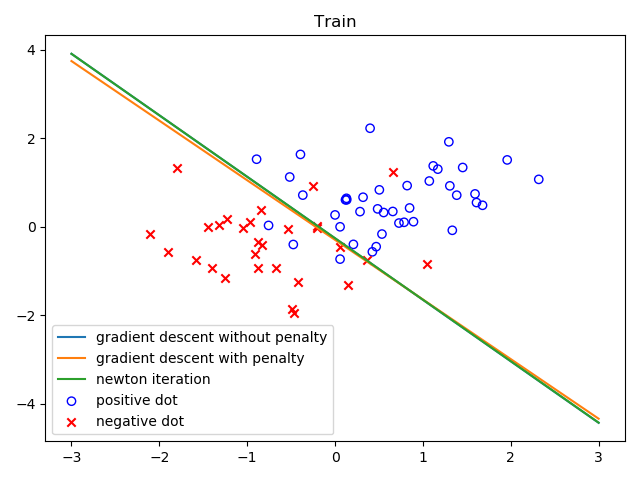
\includegraphics[width=.5\textwidth]{cov0Train.png}}\hfill
	\subfloat[特征间相互独立时测试集分类结果]{%
		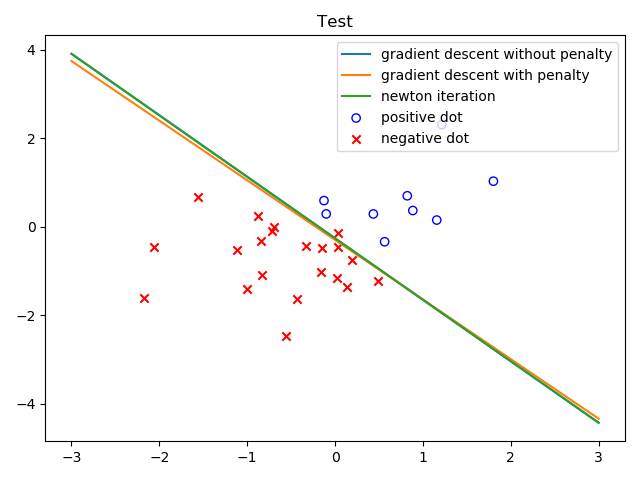
\includegraphics[width=.5\textwidth]{cov0Test.png}}
	\caption{特征相互独立时的分类结果}\label{fig:fig1}
\end{figure}

\subsection{特征不满足相互独立时的分类结果}

实验结果如图(\ref{fig:fig2})所示. 不带惩罚项的梯度下降法与带惩罚项的梯度下降法在训练集上的分类准确率均为82.86\%,牛顿迭代法在训练集上的的分类准确率为84.29\%;不带有惩罚项的梯度下降法和牛顿迭代法在测试集上的分类准确率为76.67\%,带有惩罚项的梯度下降法在测试集上的分类准确率为73.33\%.

\begin{figure}[htb]
	\centering
	\subfloat[特征间不相互独立时训练集分类结果]{%
		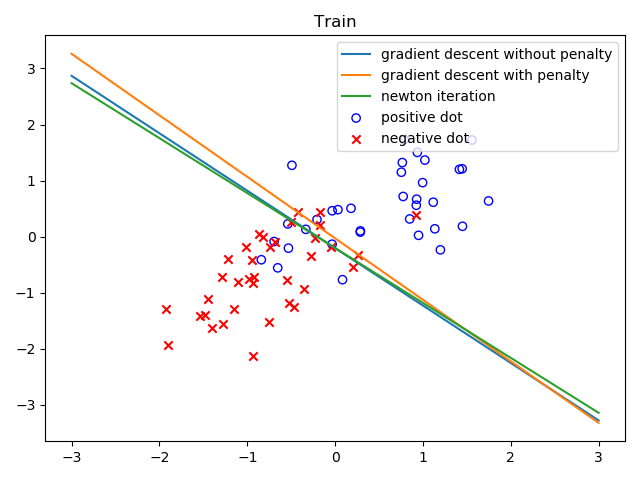
\includegraphics[width=.5\textwidth]{cov1Train.png}}\hfill
	\subfloat[特征间不相互独立时测试集分类结果]{%
		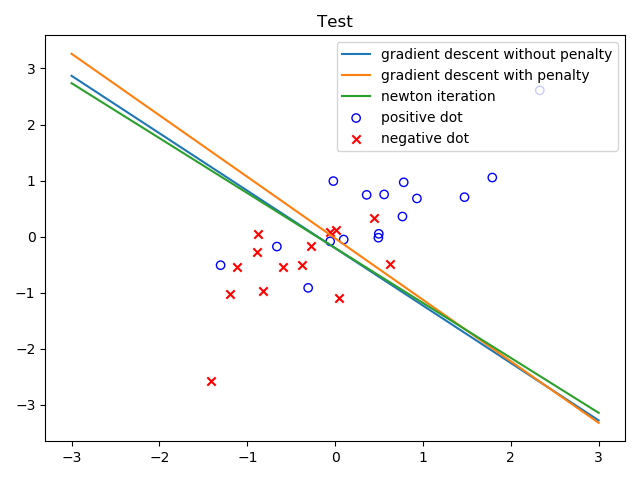
\includegraphics[width=.5\textwidth]{cov1Test.png}}
	\caption{特征相互独立时的分类结果}\label{fig:fig2}
\end{figure}

\subsection{在UCI数据集上测试结果}

由于UCI数据集banknote authentication Data Set为四维数据,所以无法画出数据在特征空间中的分布,但是得到如图(\ref{fig:fig3})所示,在训练集和测试集上的分类准确率. 在训练集上,不带有惩罚项和带有惩罚项的梯度下降法的分类准确率均为94.27\%,牛顿迭代法的分类准确率是94.38\%;在测试集上,不带有惩罚项的梯度下降法和牛顿迭代法的分类准确率均为99.51\%,带有惩罚项的梯度下降法的分类准确率为98.79\%.
\begin{figure}
	\centering
	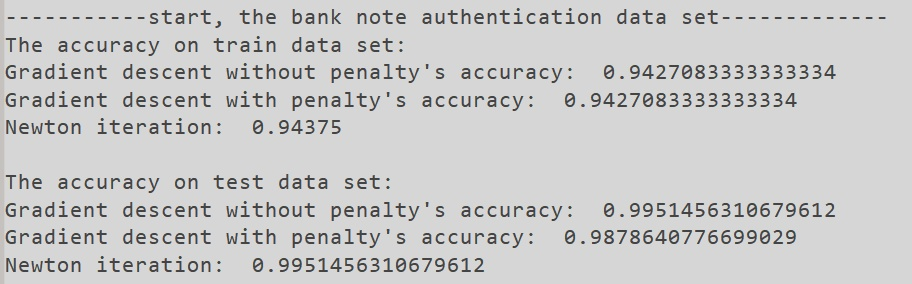
\includegraphics[width=0.7\linewidth]{owndata.png}
	\caption{在UCI数据集上测试结果}\label{fig:fig3}
\end{figure}



%\begin{figure}[htb]
%	\centering
%	\subfloat[评级A企业贷款年利率和客户流失率关系]{%
%		
\includegraphics[width=.33\textwidth]{2}}\hfill
%	\subfloat[评级B企业贷款年利率和客户流失率关系]{%
%		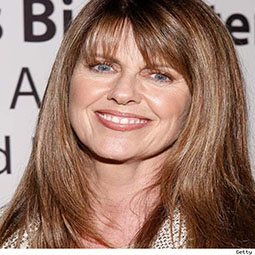
\includegraphics[width=.33\textwidth]{3}}\hfill
%	\subfloat[评级C企业贷款年利率和客户流失率关系]{%
%		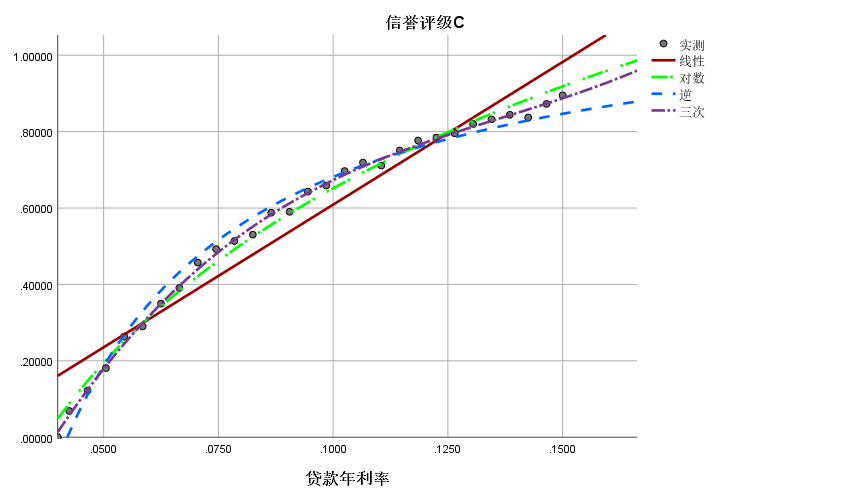
\includegraphics[width=.33\textwidth]{4}}
%	\caption{不同信誉评级的企业贷款年利率和客户流失率关系图示}\label{fig:churn_rate}
%\end{figure}

%\section{操作方法和实验步骤}
%\subsection{传输函数}
%对差分方程进行处理,求出传输函数表达式.
%\subsection{零极点分布图}
%在此基础上,使用Matlab中的zplane函数进一步画出在不同a取值情况下的零极点分布图.
%\subsection{幅频响应}
%之后使用freqz函数画出不同a取值情况下的频率响应图像.
%
%\section{实验数据记录和处理}
%\subsection{传输函数}
%根据差分方程,传输函数如下:
%$$H(z) = \frac{Y(z)}{X(z)} = \frac{z^2}{z^2-(0.5+a)z+0.5a}$$
%\subsection{零极点分布图}
%a = 0.8,0.9,1.1时,系统的零极点分布图及程序如下:
%\begin{enumerate}
%  \item 图像
%        \begin{center}
%          \includegraphics[width=0.6\linewidth]{01.jpg}
%        \end{center}
%  \item 代码
%        \lstinputlisting[language=MATLAB]{code/do.m}
%\end{enumerate}
%
%\subsection{频率响应}
%a = 0.8,0.9,1.0,1.1时,系统的频率响应函数图形及程序如下:
%\begin{enumerate}
%  \item 图像
%        \begin{center}
%          \includegraphics[width=0.6\linewidth]{02-1.jpg}
%        \end{center}
%  \item 代码
%        \lstinputlisting[language=MATLAB]{code/next.m}
%\end{enumerate}

\section{实验结论}

\begin{enumerate}
\item 数据量较大时,惩罚项对分类超平面的影响逐渐降低;
\item 牛顿迭代法与梯度下降法均可以得到较好的实验结果,分类结果较为准确;
\item 在数据特征较少时,尽管不满足特征间相互独立的条件,Logistic回归仍然可以做到较好的分类,当数据特征较多时,如果不满足特征间相互独立的条件,分类结果较差;
\item Logistics回归可以很好地解决简单的线性分类问题,而且收敛速度较快.
\end{enumerate}

\renewcommand\refname{参考文献}
 
\begin{thebibliography}{2}
\bibitem{book:li}
李航, 统计学习方法(2019.3).

\bibitem{book:zhou}
周志华, 机器学习(2016.1).

\bibitem{url:bank}
\href{http://archive.ics.uci.edu/ml/datasets/banknote+authentication}{Banknote Authentication Data Set. (2012.8) [Data set]}
\end{thebibliography}


\end{document}
